\chapter{在量子模型检测中应用TDD表示}

张量决策图(TDD)是一种基于张量网络,结合了二元决策图的表示优势的数据结构。
TDD针对于量子计算,可以有很好的空间优势,同时也可以很方便的结合过去在二元决策图的模型检测算法的优化技术。
本章将主要介绍在本文工作中使用的方法,因此将首先介绍TDD,然后介绍如何应用TDD进行模型检测并作出针对性改进,最后介绍本文工作中的软件实现。

\section{TDD简介}
TDD是一种决策图样式的数据结构,用于使用张量网络表示量子电路。
本节将从用张量网络表示量子电路开始,然后简单介绍张量网络如何转换到TDD,最后简单介绍TDD与类似表示的对比。
有关TDD的具体内容,可以参考\citep{Hong_2022}。
% 目前,TDD研究集中在开发更有效的算法来使用TDD操作和收缩张量网络。这包括开发新技术来分割张量网络,优化TDD结构,从而进一步提高基于TDD的可达性分析和模型检测算法的效率。这也是实现基于TDD的量子模型检测的主要方法。
\subsection*{TDD定义}
张量是与一组与索引序列\(I=\{x_1,\ldots,x_n\}\)相关联的多维线性映射。在量子计算中,可以假设只从\(\{0,1\}\)中取值。因此,张量定义为定义\ref{df-tensor}所示。
\begin{definition}\citep{biamonte2019lectures}
    \label{df-tensor}
    当张量只从从\(\{0,1\}\)中取值时,对于定义在索引序列\(I\)上的张量\(\phi\),其可以表示为一个字典
    \begin{align}
        \phi :{\{0,1\}}^I\rightarrow\mathbb{C}
    \end{align}
    其中\(\mathbb{C}\)为复数。
\end{definition}


因此一个向量表示为$[\alpha_0,\alpha_1]$的量子比特$x$可以描述为秩为$1$的张量$\phi_x$,其中$\phi_x\left(0\right)=\alpha_0, \phi_x\left(1\right)=\alpha_1$。具有输入比特$x$和输出比特$y$的单比特门可以表示为秩为$2$的张量$\phi_{xy}$。类似的$n$比特量子门可以表示成一个秩为$2n$的张量。在张量表示中,一般不区分输入和输出索引。只有当将张量解释为门或电路时会规定关于其信息。

张量之间最重要的运算之一是收缩(contraction)。收缩是通过对共享索引求和获得新的张量。具体来说,设 张量$\gamma_{\overrightarrow{x},\overrightarrow{z}}$ 和 $\xi_{\overrightarrow{y},\overrightarrow{z}}$ 的共享索引集 是$\overrightarrow{z}$。设收缩后的新张量为 $\phi_{\overrightarrow{x},\overrightarrow{y}}$,则其表达式如式子\ref{eq-contraction}所示。
\begin{equation}
\label{eq-contraction}
\phi_{\overrightarrow{x},\overrightarrow{y}}(\overrightarrow{a},\overrightarrow{b}) = \sum_{\overrightarrow{c} \in \{0,1\}^{\overrightarrow{z}}} \gamma_{\overrightarrow{x},\overrightarrow{z}}(\overrightarrow{a}, \overrightarrow{c}) \cdot \xi_{\overrightarrow{y},\overrightarrow{z}}(\overrightarrow{b}, \overrightarrow{c}).
\end{equation}

另一个重要的张量操作是切片(slicing),它对应于布尔函数的余因子运算。设 $\phi$ 是索引序列为 $I$ 上的张量。任取一个索引\(x\in I\),对 $\phi$ 进行关于 $x = c$ 与 $c \in \{0, 1\}$ 的切片也是一个张量 $\phi|_{x=c}$,在索引集 $I' =I/\{x\}$ 上定义如式子\ref{eq-slicing}所示。
\begin{equation}
    \label{eq-slicing}
\phi|_{x=c}(\overrightarrow{a}) := \phi(c, \overrightarrow{a})
\end{equation}
对于任意 $\overrightarrow{a} \in \{0, 1\}^n$。称 $\phi|_{x=0}$ 和 $\phi|_{x=1}$ 分别为 $\phi$ 关于 $x$ 的负切片(negative slicing)和正切片(positive slicing)。如果 $\phi|_{x=0} \neq \phi|_{x=1}$,称索引 $x \in I$ 对于 $\phi$ 是本质的(essential)。
% 同时张量满足定理\ref{lemma-tensor}中的性质。

% \begin{lemma}
%     \label{lemma-tensor}
%     对于定义在索引序列\(I\)上的张量\(\phi\),其中的每个索引\(x\in I\),都有
%     \begin{align}
%         \phi = \bar{x}\cdot \phi|_{x=0}+x\cdot \phi|_{x=1}
%     \end{align}
% \end{lemma}

张量网络是一个无向图\(G=\left(V,E\right)\)。其中顶点集$V$中的每个顶点$v$表示一个张量。边集\(E\)中每条边\(e\)代表与相邻两个张量相关联的公共索引。通过以任意顺序收缩连接的张量,可以得到一个秩为\(m\)的张量,其中\(m\)是$G$中开放边数。这个独立于收缩顺序的张量也称为该张量网络的张量表示\citep{biamonte2019lectures}。
张量网络提供了一种新的量子线路表示方法\citep{pednault2017breaking}。而当给定量子线路中所有量子门的输入和输出状态的索引值,收缩掉共享的索引,就可以得到量子电路的张量表示。


TDD是一种具有决策图和张量网络特征的数据结构\citep{Hong_2022}。它可用于表示张量,并进一步表示量子电路。与BDD(Boolean Decision Diagrams)类似,TDD是一种建立在索引顺序$I=\{x_1,\ldots,x_n\}$上的决策树模型。具体定义定义\ref{df-tdd}所示。
\begin{definition}\citep{Hong_2022}
    \label{df-tdd}
    TDD是一个建立在索引顺序$I=\{x_1,\ldots,x_n\}$上的有根节点,带权重的有向无环图,其中包括:
    \begin{align}
        \mathcal{F}=\left(V,E,index,value,low,high,w\right)
    \end{align}
    其中:
    \begin{enumerate}
        \item $V$是一个有限节点集,被划分为非终端节点$V_n$和终端节点$V_T$。用$r_{\mathcal{F}}$表示$\mathcal{F}$的唯一根节点。
        \item $E=\left\{\left(v,low\left(v\right)\right),\left(v,high\left(v\right)\right):v\in V_N\right\}$是树中所有边集合,其中$\left(v,low\left(v\right)\right)$和$\left(v,high\left(v\right)\right)$分别称为v的低边和高边,分别指向该节点索引的负切片和正切片。根结点$r_{\mathcal{F}}$具有唯一的入射边$e_{\mathcal{F}}$,该入射边没有源结点。
        \item $index:V_r\rightarrow I$将每个非终端节点分配给I中的索引。
        \item $value:V_T\rightarrow\mathbb{C}$将每个终端节点赋予一个复数值。
        \item $low$和$high$都是$V_N\rightarrow V$中的映射,它们分别为每个非终端节点指定其低边和高边后继。
        \item $w:E\rightarrow\mathbb{C}$将每条边赋予一个复数权重。特别地,$w\left(e_r\right)$称为$\mathcal{F}$的权重,并记作$w_{\mathcal{F}}$。
    \end{enumerate} 
\end{definition}


对于TDD中的一个节点$v$,如果$v$是终端节点,则$\phi\left(v\right):= value (v)$是一个秩为$0$的张量,即常数,也可以称为一个平凡TDD。如果$v$是非终端节点,则根据定义,该节点表示的张量如式子\ref{eq-non-term}所示。
\begin{align}
    \label{eq-non-term}
    \phi(v):=w_{0} \cdot \overline{x_{v}} \cdot \phi(\operatorname{low}(v))+w_{1} \cdot x_{v} \cdot \phi(h i g h(v))
\end{align}
其中$x_v=index\left(v\right),\overline{x_{v}}=1-index\left(v\right)$。而整个TDD也可以表示为:
\begin{align}
    \phi\left(\mathcal{F}\right)=w_{\mathcal{F}}\cdot\phi\left(r_{\mathcal{F}}\right)
\end{align}


\subsection*{TDD的规范与化简}
\label{sec-reduce}
根据定义得到的TDD在结构上显然比较冗余,可以进行进一步化简。具体过程是先进行规范化(normalized),让后进行化简(reduced)\citep{Hong_2022}。
其中规范化的目的是使得TDD的终端节点只包含0和1,同时将终端节点的张量值沿路径逐步上移。具体规范步骤如下:
\begin{enumerate}
    \item 如果$v$是一个非零值$value\left(v\right)\neq 1$的终端节点,则将其值设置为1,并将每个入边的权重w更改为$value\left(v\right)\cdot w$。\label{norm1}
    \item 假设v是一个非终端节点,且$\phi\left(v\right)\neq 0$。首先规范化$\phi\left.\left(low(v\right)\right)$和$\phi\left.\left(high(v\right)\right)$。完成$\phi\left.\left(low(v\right)\right)$和$\phi\left.\left(high(v\right)\right)$的规范化后。如果$\phi\left.\left(low(v\right)\right)\neq 0$,并且此时$\phi\left.\left(high(v\right)\right)=0$或$\left|w_0\right|\geq\left|w_1\right|$,则将$w$设置为$w_0$。否则,将$w$设置为$w_1$。然后更新$w_0≔w_0/w,w_1≔w_1/w$。此时完成$v$的规范化。\label{norm2}
\end{enumerate}



在完成规范化后,此时的TDD终端节点只包含0和1。可以进一步简化TDD,使得TDD只包含一个终端节点1,同时尽量使用重复出现的张量。具体简化步骤如下:
\begin{enumerate}
    \item 	合并所有值为1的终端节点。删除所有终端$0$节点,并将它们的入边重定向到唯一的终端节点,并将它们的权重重置为$0$。\label{sympl1}
	\item 将所有权重为$0$的边重定向到终端节点。如果根节点的入边权重为$0$,则终端节点成为新的根,该TDD为空。删除所有从根节点不可达的节点,以及涉及它们的所有边。\label{sympl2}
	\item 如果一个节点v的低边和高边后继相同,并且其低边和高边具有相同的权重w,则删除该节点。如果入边权重$w=0$,则将其传入边重定向到终端节点。否则,将其传入边重定向到其后继节点。\label{sympl3}
	\item 合并两个具有相同索引、相同$0$和$1$后继以及对应边上相同权重的节点。\label{sympl4}
\end{enumerate}


为了阅读简洁,下文中无特殊说明的TDD均指化简后的TDD,即reduced tensor decision diagrams。结合以上步骤,算法\ref{alg-tdd}简单展示了如何将给定的张量\(\phi\)转换为对应的TDD表示。
\begin{algorithm}
    \caption{生成张量\(\phi\)的TDD表示TDD(\(\phi\))\citep{Hong_2022}}
    \label{alg-tdd}
    \begin{algorithmic}[1]
    \Require 一个张量\(\phi\) 和对应的索引顺序\(I\)
    \Ensure \(\phi\)的TDD表示TDD(\(\phi\))
    \If{\(\phi = c\),即输入张量是一个标量}
        \State \Return 带权重$c$的平凡TDD
    \EndIf
    \State \(x \gets\) \(\phi\)在索引顺序\(I\)中最小的索引
    \State \(tdd \gets\) 一个空的TDD
    \State \(tdd.root \gets\) 一个索引为\(x\)的新节点\(v\) 
    \State \(v.low \gets\) 递归调用本算法,得到\(\phi|_{x=0}\)对应的TDD表示TDD(\(\phi|_{x=0}\))
    \State \(v.high \gets\) 递归调用本算法,得到\(\phi|_{x=1}\)对应的TDD表示TDD(\(\phi|_{x=1}\))
    \State \(tdd.weight \gets 1\)
    \State \Return \(tdd\)化简后的TDD表示
    \end{algorithmic}
\end{algorithm}


\subsection*{对比类似表示}
\label{sec-compare}
TDD是一种相对较新的数据结构,用于表示和操作张量网络。张量网络提供了量子线路更紧凑的表现形式。本小节中将对比定义\ref{df-tensor}中的张量网络TN,定义\ref{df-tdd}中的张量决策图TDD,以及QMDD\citep{1623982}三种表示的效率。

QMDD(Quantum Multiple-Valued Decision Diagrams),即量子多值决策图提供了一种紧凑而系统的方法来描述量子过程。目前QMDD已有效地用于量子电路的合成\citep{niemann2020advanced}和和验证任务
\citep{burgholzer2020verifying,burgholzer2020advanced}。
图\ref{fig:qmdd-basic}展示了一个矩阵到最终QMDD的一个过程。
\begin{figure}[htbp]
    \centering
    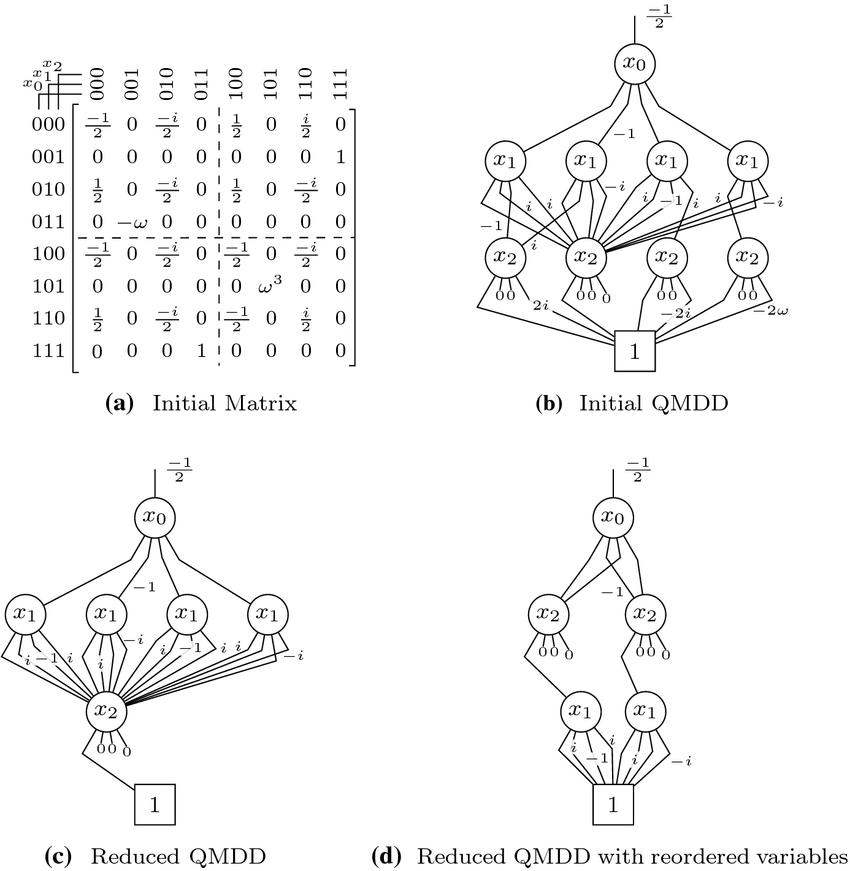
\includegraphics[height=10cm]{Img/QMDD-intro}
    \caption{一个QMDD的示例}
    \label{fig:qmdd-basic}
\end{figure}

可以看到QMDD和TDD的相似点有:
\begin{enumerate}
    \item 二者都存在唯一的终端顶点,值为1。该终端顶点没有出边。
    \item 二者都有唯一一个顶点作为起始顶点,它有一个单独的入边,该入边本身没有源顶点。
    \item 二者中的每条边(包括指向起始顶点的边)都有一个关联的复数值权重。
    \item 二者中的索引都按一定顺序排列,并且都满足以下两条规则:
    \begin{enumerate}[label=\roman*)]
        \item 每个索引在从起始顶点到终端顶点的每条路径上最多出现一次。
        \item 来自索引排序低的非终端顶点的边指向索引排序高的非终端顶点或终端顶点。
    \end{enumerate}
    \item 二者都尽量复用节点,即没有两个标记索引相同的非终端顶点有相同的出边集(即连接节点和边权重都一致)。
\end{enumerate}

QMDD和TDD主要不同的在于QMDD结构中,每个非终端节点连接有四个后继节点。
而在TDD结构中,每一个非终端节点分别连接着两个后继节点。
因此从原理上讲,如果采用相同的排序规则,量子电路的TDD表达方式的节点数大约是其QMDD表达方式节点数的两倍。但由于它们都拥有相同数目的加权边并记录了相同数量的权值(即复数)。此时TDD表达方式所需的内存空间与QMDD表达方式所需的内存空间持平。

虽然TDD的表示形式和QMDD紧凑程度相近。
但是TDD非常灵活,可以轻松与张量网络中的一些优化技术结合以进一步提高其表现。


图\ref{fig:tdd-compare}是\cite{Hong_2022}中展示的目前各种比较成熟的表示方法下模拟量子电路的时间对比。其中TDD No Part指的是不对电路进行拆分优化的方法。TDD part I 和TDD part II是两种的张量网络中的优化技术。
QMDD指的是Quantum Multiple-valued Decision Diagrams。
TN表示方法使用了google的tensor network\citep{roberts2019tensornetwork}。
从图\ref{fig:tdd-compare}可以看到,两种TDD的优化方案都是时间消耗最少的。不使用拆分优化的TDD No Part与QMDD时间接近。而当比特数少于10时,TN的时间少于TDD No Part,但随着比特数增加,TN的用时快速超过TDD No Part。
因此TDD相比其他表示方式有一定优势。这是本文工作研究中选择TDD作为主要技术的重要原因。

\begin{figure}[!htbp]
    \centering
    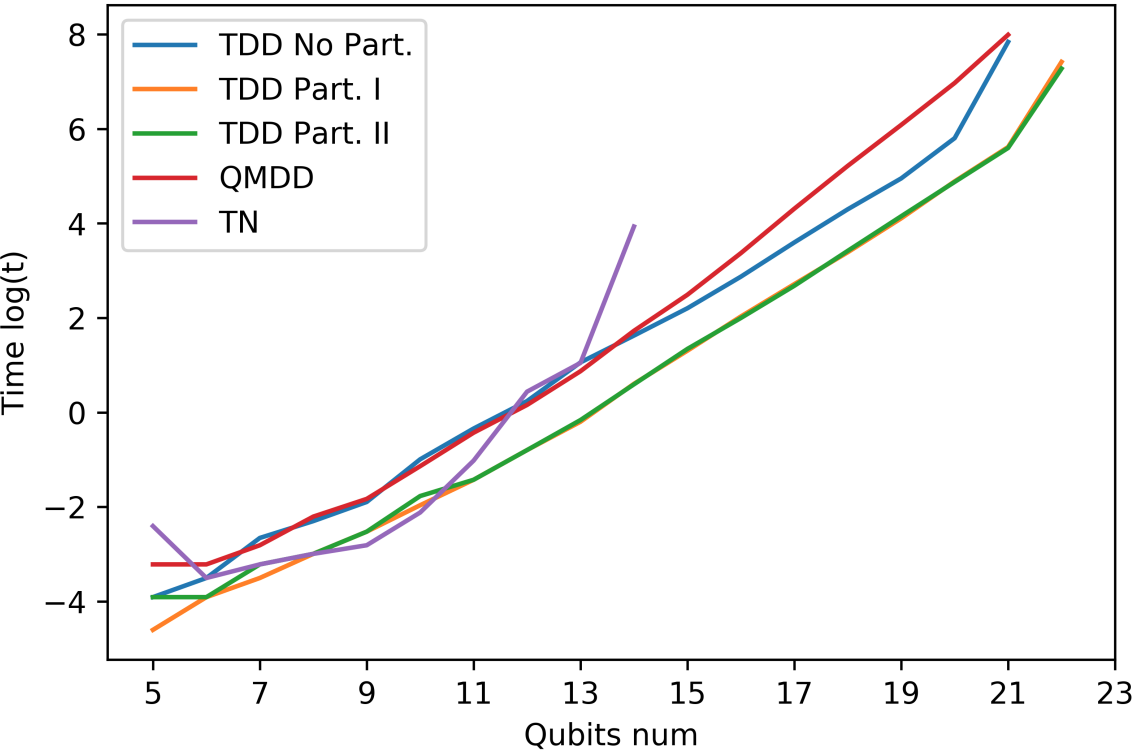
\includegraphics[height=8cm]{Img/tdd-compare.pdf}
    \caption{对QFT电路,TDD与TN,QMDD表示的比较\citep{Hong_2022}}
    \label{fig:tdd-compare}
\end{figure}

\section{将量子系统建模为量子迁移系统}

在\ref{sec-transition}节中介绍了跃迁系统,其中定义\ref{def-model-q}给出了量子跃迁系统的简单定义。这里简单回顾一下。对于一个希尔伯特空间$\mathcal{H}$ 。基于 $\mathcal{H}$ 的量子转移系统 $\mathcal{M}$ 可以表述为四元组 $(\mathcal{H}, S, \Sigma, \mathcal{T})$,这里 $S$ 作为 $\mathcal{H}$ 的一个封闭子空间,被定义为初始空间。$\Sigma=\{\sigma_1,\ldots,\sigma_m\}$ 是一系列符号集合,$\mathcal{T}=\{\mathcal{T}_\sigma, \sigma \in \Sigma\}$ 则代表对 $\mathcal{H}$ 执行的一组量子操作。


\begin{example}
    一个单量子比特的系统可能遭受两种潜在的噪声影响:比特位翻转和相位翻转。如果不能准确判断会发生哪一种噪声,这样的系统可以被表达为一个量子转移系统 $\mathcal{M}=\big(\mathcal{H}_2,S,\{1,2\},\{\mathcal{T}_1,\mathcal{T}_2\} \big)$,这里 $S$ 代表 $\mathcal{H}$ 中的一个子空间,$\mathcal{T}_1=\{\sqrt{p}I, \sqrt{1-p}X\}$ 和 $\mathcal{T}_2=\{\sqrt{p}I, \sqrt{1-p}Z\}$。 $I,X,Z$ 分别代表恒等矩阵、Pauli $X$ 矩阵和Pauli $Z$ 矩阵。
\end{example}
\begin{example}
    \label{ex-image-grover}
    量子线路也可以表达为一个量子迁移系统。图\ref{fig:grover}展示了实现两量子比特 Grover 迭代的电路 \citep{Grover_1996},这是 Grover 算法的一个基本过程,用于找到布尔函数 $f(x)=1$ 的解。该类算法需要验证的属性是能否始终进入布尔函数解所在的子空间。
    对于该电路,第一个 CCX 门表示搜索用的oracle,实现了$ O\ket{x}\ket{y}=\ket{x}\ket{f(x)\oplus y}$,其中 $f(x)=x_1 \wedge x_2$。因此,该电路oracle的解是\(00\) 。其他门实现了一个补$2\ket{\psi}\bra{\psi}-I$,其中$\ket{\psi}=\frac{1}{\sqrt{2}^{n}}\sum_{i=0}^{2^n-1}\ket{i}$。给定输入状态 $\ket{++-}=\frac{1}{2}\sum_{i=0}^3\ket{i}\ket{-}$,电路首先将状态变为 $\frac{1}{2}\sum_{i=0}^2 \ket{i}\ket{-}-\frac{1}{2}\ket{11}\ket{-}$,然后变为 $\ket{11}\ket{-}$。对于状态空间 $S=span\{\ket{++-},\ket{11-}\}$。当目前系统状态 $\ket{\varphi} \in S$,下一步系统状态总会在 $S$ 中。

    因此该系统可以表示为量子迁移系统 $(\mathcal{H}_8, S, {1}, \mathcal{T})$ 进行建模,其中 $\mathcal{T}_1 = {(2\ket{\psi}\bra{\psi}-I) O}$,需要检查的属性是$\mathcal{T}_1(S)=S$。
    \begin{figure}[!htbp]
        \centering
        \includegraphics[height=4cm]{Img/cir_grover.pdf}
        \caption{Grover\_3的量子线路图}
        \label{fig:grover}
    \end{figure} 
\end{example}
\section{基于TDD表示的子空间算法}
\subsection{子空间的分解}
在\ref{sec-logic}节中介绍了量子逻辑中的原子命题用希尔伯特空间中的子空间表示。
因此在量子模型检测中,需要用到子空间的表示。而一种比较方便的表示子空间的办法是将子空间表示为一组基态。
给定子空间投影算子的矩阵形式,如果有一个非零的列向量,那么在该向量的方向上就可以找到一个基向量。然后,通过正交化过程,可以递归地找到原始子空间的一组正交基向量。


但是使用矩阵表示进行所有列的遍历会遇到很高的复杂度。而通过使用子空间投影算子的TDD表示,就可以可以容易地找到第一个非零列。
具体方法是寻找该TDD表示的最左侧非零路径。
通过这种图的方法避免了在计算过程中需要显式表示相应的向量,也减少了0复杂度​​。
综上所述,算法\ref{alg-basis_dec}给出了一个计算子空间的一组计算基的方法。在此算法基础上,可以给出根据当前系统状态计算下一步系统状态的算法\ref{alg-image}.
\begin{algorithm}
\caption{给出投影算子$P$的一组正交基}
\label{alg-basis_dec} 
\begin{algorithmic}[1]
    \Require 子空间$S$的TDD形式投影算子$P=P_S$ 
    \Ensure $P$的一组正交基分解$B$
    \State $B\gets \{\}$
    \If{\(P\) 是空的} 
        \Return \(B\)
    \Else
        \State \(\ket{i} \gets\) TDD表示\(P\)中最左侧非零路径所表示的列号\(i\)
        \State \(\ket{u_i}\gets\) 由在TDD表示\(P\) 中具有列号 \(\ket{i}\) 的路径表示的状态
        \State \(\ket{v_i} \gets \frac{\ket{u_i}}{\|\ket{u_i}\|}\)
        \State \(P \gets P - \ket{v_i}\bra{v_i}\)
        \State \(B' \gets \) 递归调用本算法,得到新的$P$的计算基分解
        \State \(B \gets B \cup \{\ket{v_i}\} \cup B'\)
    \EndIf
    \State \Return \(B\)
\end{algorithmic}
\end{algorithm}

\begin{example}
    \label{ex-image-sub}
    例子\ref{ex-image-grover}将Grover算法的电路建模为量子迁移系统。其中用到了子空间$S=span\{\ket{++-},\ket{11-}\}$。相应投影算子 $P$ 的矩阵和 TDD 表示如图 \ref{fig:P} 所示。
    根据该TDD表示求解原子空间的基的过程如下:
    \begin{enumerate}
        \item 应用图算法,得到最左侧路径对应于 $(x_1,x_2,x_3,y_1,y_2,y_3)=(0,0,0,0,0,0)$,这意味着投影算子的第一列非零。
        \item 遍历所有 $(x_0,x_1,x_2)=(0,0,0)$ 的路径,得到向量 $\ket{v_1}=\frac{1}{6}[1,-1,1,-1,1,-1,0,0]$。
        \item $\ket{v_1}$标准化为 $\ket{v_1}=\frac{1}{\sqrt{3}}(\ket{00}+\ket{01}+\ket{10})\ket{-}$。
        \item 设 $P'=P-\ket{v_1}\bra{v_1}$。那么 $P'$ 等于 $\ket{11-}\bra{11-}$。
        \item 对 $P'$ 重复上述的过程,获得 另一组基$\ket{v_2}=\ket{11}\ket{-}$,此时TDD为空。因此 ${\ket{v_1},\ket{v_2}}$ 是子空间 $S$ 的一个基。
    \end{enumerate}
\end{example}
\subsection{子空间的并}
在\ref{sec-connect}节中介绍了量子逻辑中的连接词。
其中子空间之间的包含理解为量子逻辑的蕴含;子空间 的正交补理解为量子逻辑的否定;子空间的交理解为量子逻辑的合取;些子空间的并理解为量子逻辑的析取。其中最复杂的是子空间的并。本小节主要讨论在TDD表示下子空间的并。

设 $S=S_1\vee S_2$ 为两个子空间 $S_1,S_2$ 的并集。假设 $B_1=\{\ket{\psi_{11}},\cdots,\ket{\psi_{1k}}\}$ 和 $B_2=\{\ket{\psi_{21}},\cdots,\ket{\psi_{2l}}\}$ 分别是 $S_1$ 和 $S_2$ 的一组正交基。子空间$S$的一组正交基$B$可以通过格拉姆-施密特正交化方法(Gram–Schmidt process)计算而来,具体方法如下。
\begin{enumerate}
    \item 令 $B=B_1$,并定义 $P=\sum_{j=1}^{k}{\ket{\psi_{1j}}\bra{\psi_{1j}}}$。
    \item 遍历$B_2$ 中的基向量。假设当前向量为 $\ket{\psi_{2j}}$。计算 $\ket{u_j}=\ket{\psi_{2j}}-P\ket{\psi_{2j}}$ 并将其标准化为 $\ket{v_j}=\frac{\ket{u_j}}{|\ket{u_j}|}$。
    \item 如果 $\ket{v_j}$ 为 0,则考虑下一个向量;否则,此时它与 $P$ 正交,将其添加到 $B$ 中。同时,还将 $P$ 更新为 $P+\ket{v_j}\bra{v_j}$。
    \item 重复上述过程直到遍历完 $B_2$ 中的所有元素。此时$B$ 将成为 $S$ 的一个基,$P$ 将成为到 $S$ 的投影算子。
\end{enumerate}

这个过程展示了如何从一组生成向量开始,通过计算和正交化过程,构建出一个复合空间的正交归一化基。在量子计算和量子信息中,这种方法特别有用,因为它允许准确地描述和操控量子态的子空间。

\begin{example}
    例子\ref{ex-image-grover}中对Grover 3电路建模,例子\ref{ex-image-sub}对涉及的子空间进行了分解。考虑分解的逆过程,设 $P_1,P_2$ 为两个一维子空间 $S_1,S_2$ 的投影算子,分别由 $B_1=\{\ket{++-}\}$ 和 $B_2=\{\ket{11-}\}$ 生成。显然,$P_1=\ket{++-}\bra{++-}$。将 $B_1$ 完善为 $S=S_1\vee S_2$ 的一个基。计算得到$\ket{u}=\ket{11-}-P_1\ket{11-}=\ket{11-}-\frac{1}{4}\ket{++-}=[-\frac{1}{4},\frac{1}{4},-\frac{1}{4},\frac{1}{4},-\frac{1}{4},\frac{1}{4},\frac{3}{4},-\frac{3}{4}]^T$,可以被标准化为 $\ket{v}=-\frac{1}{2\sqrt{3}}(\ket{00}+\ket{01}+\ket{10}-3\ket{11})\ket{-}$。那么 $B=\{\ket{++-},\ket{v}\}$ 是一个正交归一化基,且 $P=P_1+\ket{v}\bra{v}$ 是相应的投影算子。
\end{example}
\section{计算一步迁移}
结合子空间的分解算法,可以给出对于量子系统的一步映射算法,具体如\ref{alg-image}所示。
\begin{algorithm}
\caption{基于迁移系统的一步映射算法}
\label{alg-image}
\begin{algorithmic}[1] % The optional argument [1] enables line numbering
\Require 一个量子迁移系统 $(\mathcal{H},S,\Sigma,\mathcal{T})$, 其中转移关系$\mathcal{T}=\{\mathcal{T}_\sigma\mid \sigma\in \Sigma\}$,  $\mathcal{T}_\sigma=\{E_{\sigma,j_\sigma}\}$
\Ensure 系统下一步状态$\mathcal{T}(S)$的投影算子$P$
\State $P \gets 0$ 
\State $B \gets $调用算法\ref{alg-basis_dec},得到$S$的计算基分解
\State $K \gets \cup_{\sigma,j_\sigma}\{E_{\sigma,j_\sigma}\}$
\For{$\ket{\psi}$ \textbf{在} $B$, $E$ \textbf{在} $K$}
    \State $\ket{\phi} \gets $收缩\(\ket{\psi}\)和\(E\)所有相同索引
    \State $P=P \vee \text{span}\{\ket{\phi}\}$
\EndFor
\State \Return $P$ 
\end{algorithmic}
\end{algorithm}

在此基础上,可以计算该量子迁移系统$(\mathcal{H},S,\Sigma,\mathcal{T})$的可达空间。具体方法如下:
\begin{enumerate}
    \item 初始化可达空间为\(R = S\),并计算可达空间的投影算子\(P_{R}\)。
    \item 调用算法\ref{alg-image},计算系统$(\mathcal{H},S,\Sigma,\mathcal{T})$下一步状态\(S'=\mathcal{T}(S)\)。
    \item \label{it-be}调用算法\ref{alg-basis_dec},分解子空间得到\(S'\)的一组基\(B = \{\ket{\psi_{1}},\cdots,\ket{\psi_{n}}\}\)。同时初始化一个空的状态空间$S''$。
    \item 遍历\(B\)中的基,假设当前向量为\(\ket{\psi_{i}}\),计算得到\(\ket{u_i}=P\ket{\psi_{i}}\),并标准化为$\ket{v_j}=\frac{\ket{u_j}}{|\ket{u_j}|}$。
    \item \label{it-end}当$\ket{v_j}$为0时,考虑下一个向量;否则,此时$\ket{v_j}$与P正交,将该向量张开的空间并到子空间$S''$中,即$S''=S''\vee span\{\ket{v_j}\}$。同时更新可达空间$R=R\vee span\{\ket{v_j}\}$,即将 $P$ 更新为 $P+\ket{v_j}\bra{v_j}$。
    \item 遍历结束后,如果$S''$为空,说明该量子系统的可达空间已经收敛,即此时的$R$就是系统的可达空间。否则用$S''$作为量子系统的初态,计算迁移系统$(\mathcal{H},S'',\Sigma,\mathcal{T})$的下一步状态,并重复上述\ref{it-be}到\ref{it-end}的过程。
\end{enumerate}

\section{针对模型检测的改进}
\label{sec-optimize}
本文工作的主要目的是借助TDD数据结构,构建能快速计算量子模型检测中可达问题的方案。本文工作的主要挑战在于尽可能减少程序的运行时间以及空间资源。为此,需要采用一系列方法来开发更有效的算法,以优化TDD操作和收缩张量网络。其中包括开发新技术来分割电路和优化TDD结构。下面简单介绍一下具体改进方法。
\subsection*{索引顺序的调整}
\label{contraction}在BDD中,索引的顺序很重要。因为索引顺序会直接影响BDD的大小。一个良好的变量顺序可以使得BDD比一个糟糕的变量顺序小得多。图\ref{fig:bdd-compare}的了两张图都表示了布尔函数$f (x1,...,x8)=x1x2+x3x4+x5x6+x7x8$,但图\ref{fig:bdd-good}的结构更简单。其中图\ref{fig:bdd-bad}的索引顺序为\{x1,x3,x5,x7,x2,x4,x6,x8\},图\ref{fig:bdd-good}的索引顺序为\{x1,x2,x3,x4,x5,x6,x7,x8\}。找到一个好的索引顺序是一个NP问题。在工程实现中,目前只能通过小规模电路上寻求规律,然后在更大规模电路中应用较优顺序。
% \textcolor{red}{目前也有一些研究借助xxx机器学习算法,寻找收缩的最佳序列\citep{zhang2024quantum}}
\begin{figure}[!htbp]
	\centering
	\begin{subfigure}[b]{.4\textwidth}
        \centering
        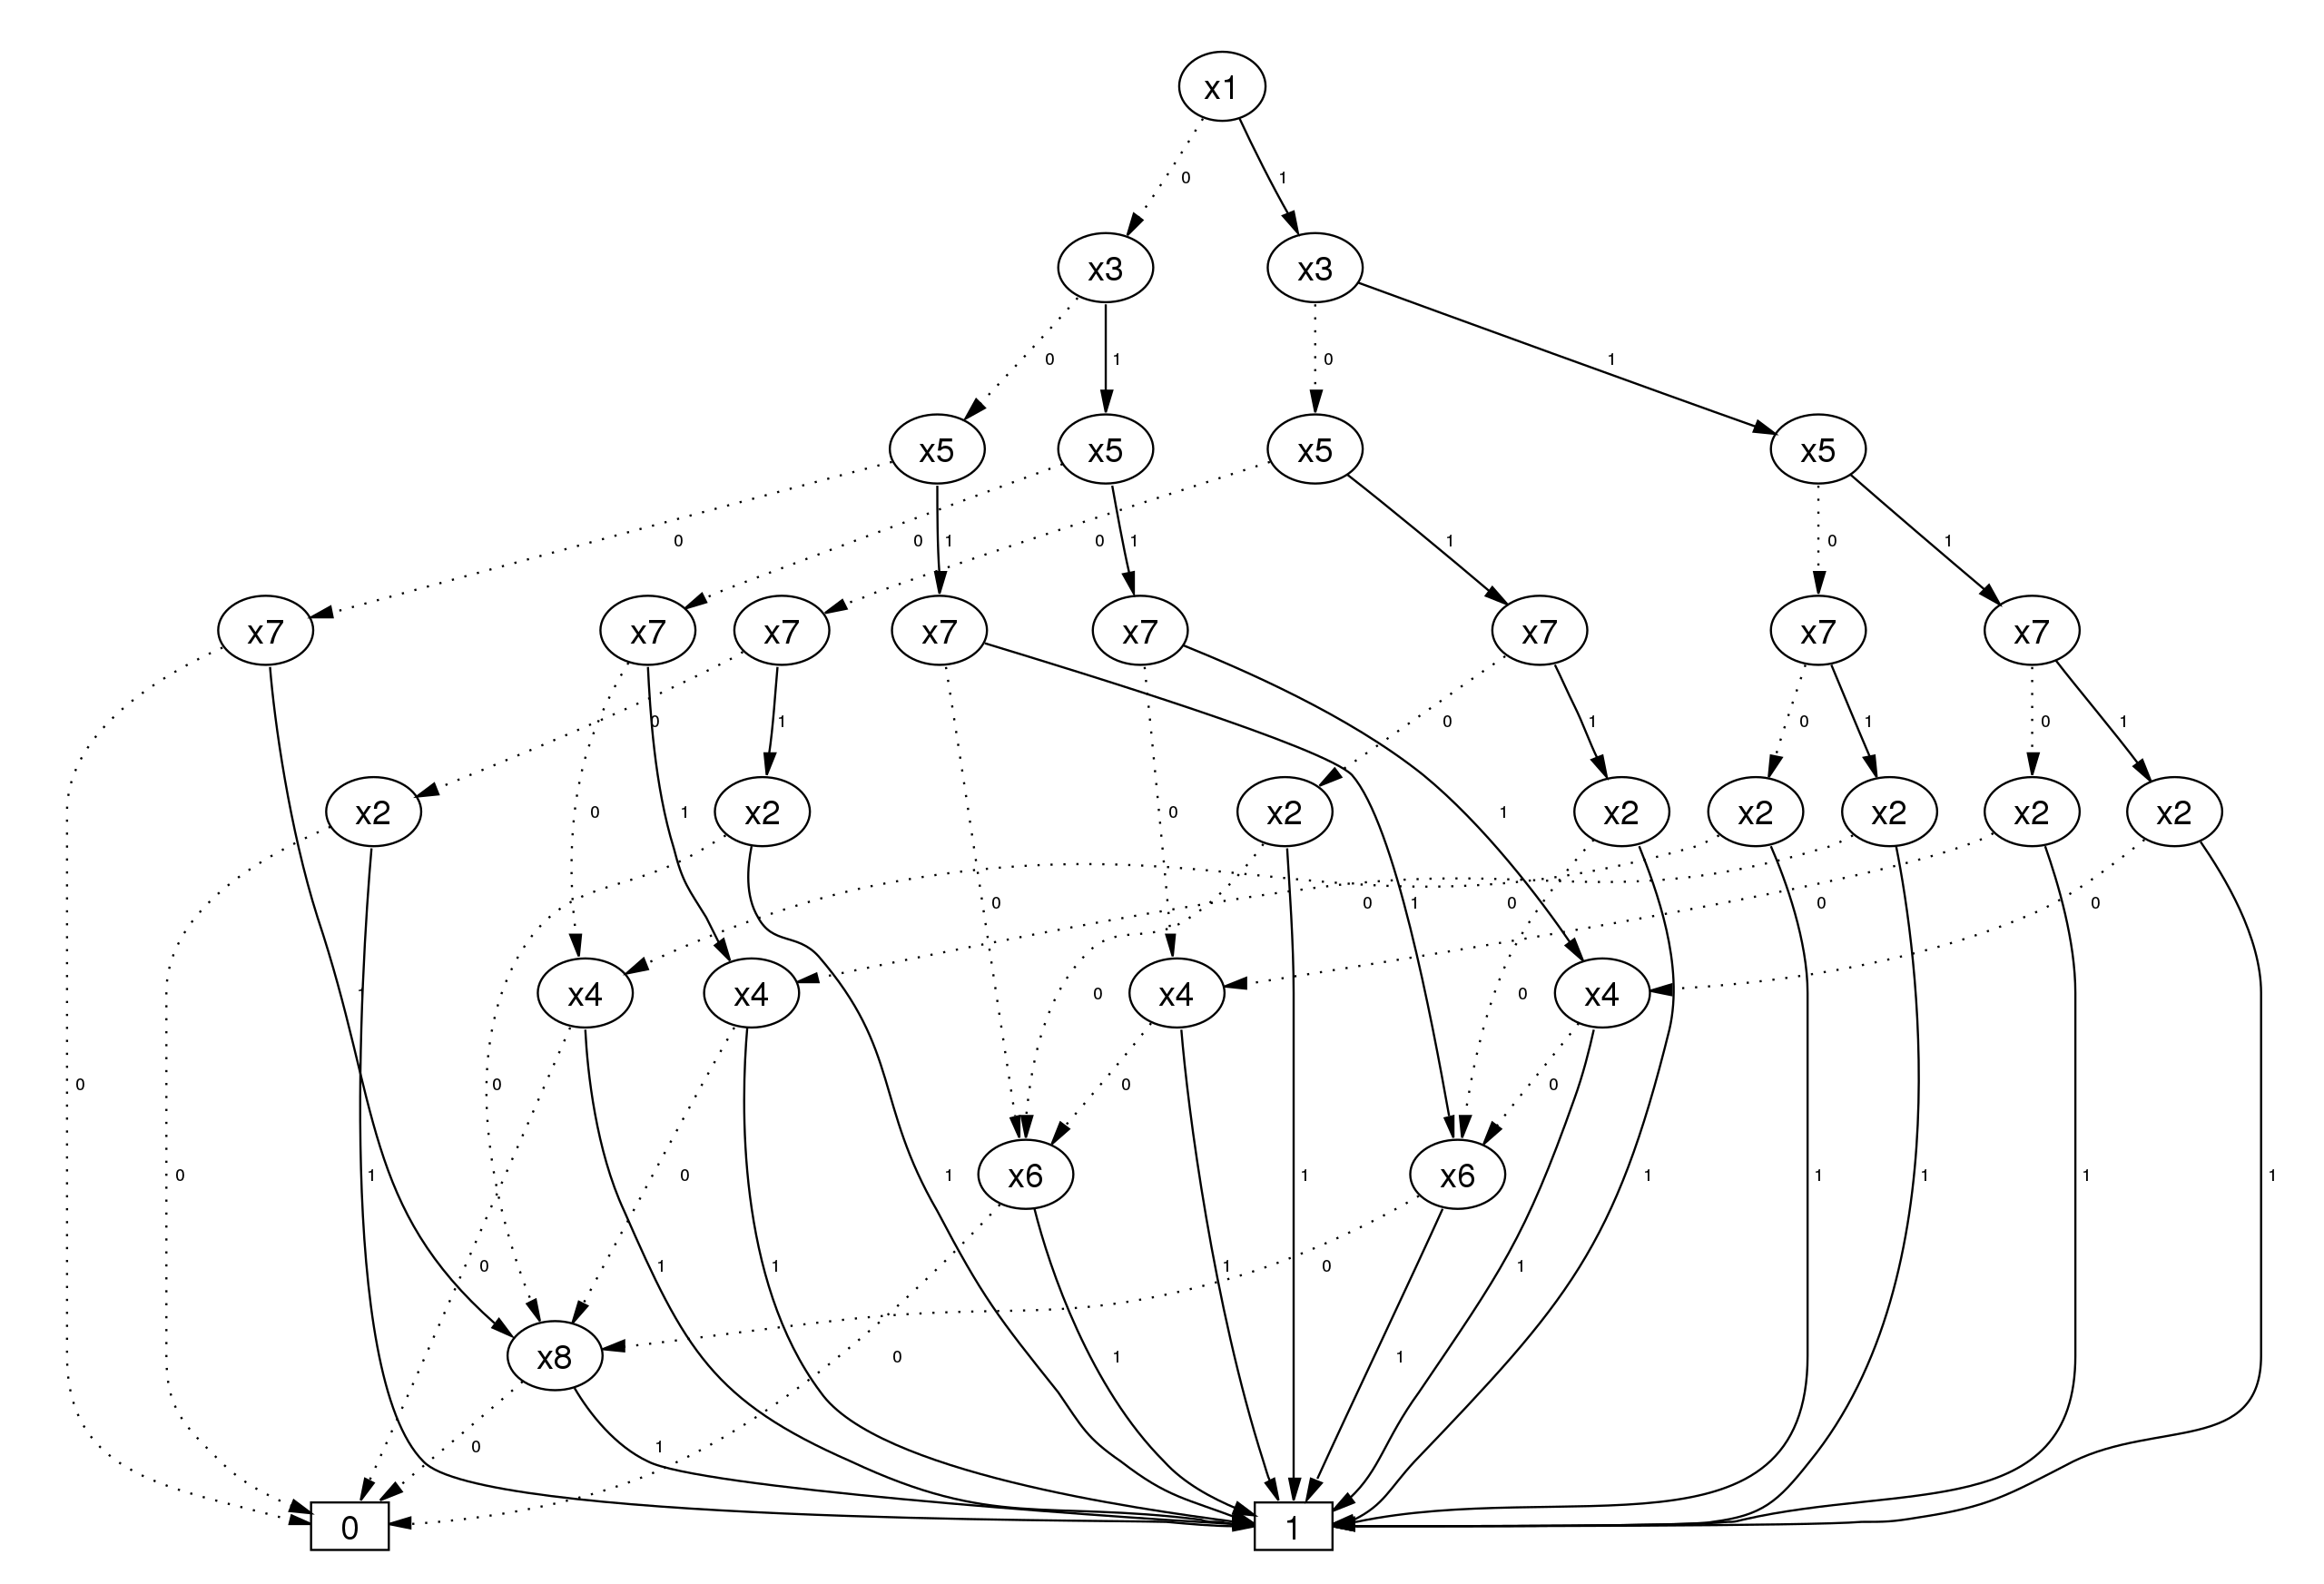
\includegraphics[height=6cm]{Img/BDD_Variable_Ordering_Bad.svg.pdf}
		\caption{索引顺序为\{x1,x3,x5,x7,x2,x4,x6,x8\}}
		\label{fig:bdd-bad}
	\end{subfigure}
    \qquad
	\begin{subfigure}[b]{.4\textwidth}
        \centering
        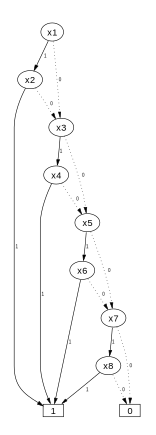
\includegraphics[height=6cm]{Img/BDD_Variable_Ordering_Good.svg.pdf}
		\caption{索引顺序为\{x1,x2,x3,x4,x5,x6,x7,x8\}}
		\label{fig:bdd-good}
	\end{subfigure}
	\caption{布尔函数$f (x1,...,x8)=x1x2+x3x4+x5x6+x7x8$在不同索引顺序下的BDD\citep{wiki:bdd}}
	\label{fig:bdd-compare}
\end{figure}

\subsection*{addition的电路拆分方案}
\label{addition}关于常用的量子线路划分方法,
第一种被称为addition\citep{chen2018classical}。将量子电路视为张量网络,首先将一个量子电路C转换成无向图G。G中的每个节点表示量子电路的一个索引,并且如果它们是相同门的输入或输出索引,则在G中连接两个节点。并且当满足以下两个条件之一时输入和输出索引不变:
\begin{itemize}
	\item 是对角线量子门的输入和输出索引;
	\item 是受控门的控制比特位的输入和输出索引。
\end{itemize}
在得到无向图后,就可以通过对连通度高索引进行张量切片,从而对量子电路进行划分。 
\begin{example}
    图\ref{fig:addition}展示了图\ref{fig:grover}中Grover\_3电路图的索引链接图。该图描述了量子电路的连通性,通过选择图中连通度最大的索引可以对电路进行分割。因此选择图中连通度较大的$x_1^1,x_1^3x_2^1$可以对电路进行较好的划分。
 
\begin{figure}[!htbp]
	\centering
	\includegraphics[height=6cm]{Img/cir_index_graph.pdf}
	\caption{Grover\_3的索引连接图}
	\label{fig:addition}
\end{figure} 
\end{example}

\subsection*{contraction的电路拆分方案}
另一种常用的电路划分方法成为contraction。该方法是\ref{sec-compare}小节中的TDD part I的延申。在这一方法中,将量子电路划分为若干个较小的部分,其收缩等于原始电路。应用两个预设整数参数$k1$和$k2$,将电路划分为若干小电路。其中每个小电路涉及最多$k1$个量子比特,并且与至多跨越不同部件的$k2$个多比特门相连。
\begin{example}
    图\ref{fig:contraction}展示了对Bit flip电路进行k1=3,k2=2的拆分结果。
\begin{figure}[!htbp]
	\centering
	\includegraphics[height=7cm]{Img/cir_contraction.pdf}
	\caption{对Bit flip电路进行contraction的拆分}
	\label{fig:contraction}
\end{figure} 
\end{example}



\subsection*{基于窗函数对TDD分割}
按照 \citep{narayan1996partitioned} 中关于经典模型检测方法的讨论,可以设计基于TDD的划分法。即利用布尔函数将一个大张量细分成若干个小张量的优化方法。设 $\varphi$ 是一个含有 $n$ 个索引的张量。从 $\set{0,1}^n$ 到 $\set{0,1}$ 的集合中选取一系列窗口布尔函数 (window boolean function)$\{w_1,\cdots, w_k\}$,这些函数对于同一输入,始终满足以下条件: 
\begin{itemize}
    \item $w_1+\cdots +w_k=1$
    \item 对任意 $i \neq j$,$w_i \cdot w_j = 0$
\end{itemize} 
因此可以看到对于一个索引$a$,有且只有一个窗口函数$w_i (a) = 1$,其他窗口函数都为$0$。
对一个张量$\varphi$,令$\varphi_i=\varphi \cdot w_i$。此时如果 $w_i(a)=1$,则$\varphi(a)=\varphi_i(a)$ ;而当$w_i(a)=0$,则$\varphi_i(a)=0$,此时存在另一个窗口函数使得$w_j(a)=1$,$\varphi(a)=\varphi_j(a)$ 。
进而,可以得出 $\varphi = \varphi_1+ \cdots +\varphi_k$。基于这样的张量划分方法,也可以对TDD进行划分。

\begin{example}
    以例子\ref{ex-image-sub}中的
    量子态 $\ket{v_1}=\frac{1}{\sqrt{3}}(\ket{00}+\ket{01}+\ket{10})\ket{-}=\frac{\sqrt{2}}{\sqrt{3}}\ket{0}\ket{+}\ket{-}+\frac{1}{\sqrt{3}}\ket{1}\ket{0}\ket{-}$ 作为示例。将 $q_0$ 量子比特看作是一个布尔变量,设$w_1=\bar{q_0}$ 和 $w_2=q_0$。窗口函数$w_1+w_2=1$,并且互斥。 $\ket{v_1}\cdot w_1$ 与 $\ket{v_1} \cdot w_2$ 分别代表(非标准化的)状态 $\frac{\sqrt{2}}{\sqrt{3}}\ket{0}\ket{+}\ket{-}$ 和 $\frac{1}{\sqrt{3}}\ket{1}\ket{0}\ket{-}$。$\ket{v_1}$ 的TDD表示及其窗口函数分割的TDD可在图\ref{fig:tdd-split} 中查看。
    \begin{figure}
    \centering
	\begin{subfigure}[b]{.3\textwidth}
        \centering
        \includegraphics[height=6cm]{Img/tdd_proj.pdf}
		\caption{$\ket{v_1}$的TDD表示}
        \label{fig:tdd-split-a}
	\end{subfigure}
	\begin{subfigure}[b]{.3\textwidth}
        \centering
        \includegraphics[height=6cm]{Img/tdd_proj_a0.pdf}
		\caption{$\ket{v_1}$在$w_1=\bar{q_0}$下的TDD表示}
	\end{subfigure}
    \quad
    \begin{subfigure}[b]{.3\textwidth}
        \centering
        \includegraphics[height=6cm]{Img/tdd_proj_a1.pdf}
		\caption{$\ket{v_1}$在$w_2=q_0$下的TDD表示}
	\end{subfigure}
    
    \caption{$\ket{v_1}=\frac{\sqrt{2}}{\sqrt{3}}\ket{0}\ket{+}\ket{-}+\frac{1}{\sqrt{3}}\ket{1}\ket{0}\ket{-}$的TDD表示与窗口函数分解}
    \label{fig:tdd-split}
    \end{figure}
\end{example}
\subsection*{用子空间近似TDD表示$\ket{\psi}$}
通过上述方法的优化,最终得到的TDD可能依然偏大。在很多实际应用中,对子空间进行一个合理的过度估计已足够,这与经典案例中的做法相似 \citep{Cho_1996,lin2014parallel,Wang+farside_iccad03}。
针对特定量子态 $\ket{\psi}$,能够通过包含它的适当子空间来近似 $\ket{\psi}$。
例如,假设已通过张量加法或窗口函数分割将量子态分为 $\ket{\psi} = \ket{\psi_1}+\ket{\psi_2}$。于是,可以通过 $span\{\ket{\psi_1},\ket{\psi_2}\}$ 子空间近似地表示 $\ket{\psi}$。

进一步地,也可以对量子态 $\ket{\psi}$ 进行张量积估计。即找到一系列张量积态 $\ket{\psi_1},\cdots, \ket{\psi_k}$,使得 $\ket{\psi}$ 位于它们张成的空间之内。这样,便能够计算出一个更大系统的映射。但这种方法的成本在于过估计子空间的维度可能会过大。给定量子态 $\ket{\psi}$,若 $\ket{\psi}=\sum_{j=0}^{2^{k-1}-1}{\ket{j}\ket{\phi}\ket{\gamma_j}}$,认为它的第 $k$ 个量子比特是可分割的。对于每个态 $\ket{\psi}$,首先探查是否存在可分割的量子比特。若存在,提取出相应的态并移除该量子比特;否则,将采用那些振幅非零的计算基态进行估计。
\begin{example}
    再次以例子\ref{ex-image-sub}中的
    量子态$\ket{v_1}=\frac{1}{\sqrt{3}}(\ket{00}+\ket{01}+\ket{10})\ket{-}$ 为例。图 \ref{fig:tdd-split-a}给出了该量子态的TDD表示。
可以发现其第三个量子比特$q_2$是可分割的,即所有的$q_0$,$q_1$都会经过同样的$q_2$结点。$q_2$对应的量子态为 $\ket{-}$。在移除这个量子比特后,得到 $\ket{\psi}=\frac{1}{\sqrt{3}}(\ket{00}+\ket{01}+\ket{10})$,该态属于子空间 $span\{\ket{00},\ket{01},\ket{10}\}$。从而为态 $\ket{v_1}$ 找到了一种张量积的近似表示 $\{\ket{00-},\ket{01-},\ket{10-}\}$。
\end{example}

\section{软件系统实现}
为了实现软件的高效运行,模块化设计至关重要。每个模块在软件系统中扮演着关键角色,并且具有特定的功能和目的。以下是本次毕业设计中软件必须包含的模块及其重要性的说明:
\begin{itemize}
    \item \textbf{输入处理模块}:该模块的主要职责是处理输入数据,例如接收用OpenQASM格式编写的量子算法代码。其核心功能是将这些代码转换为TDD表示形式。鉴于当前存在多种量子编程语言,此模块的模块化处理能够显著提升系统的灵活性和兼容性。
    \item \textbf{内存管理模块}:本模块负责管理TDD节点的存储和维护。当创建新的TDD节点时,它会运用哈希算法与现有节点进行对比,以避免重复创建相同节点。这种方法不仅减少了内存占用,还提高了处理效率。
    \item \textbf{TDD基础模块}:该模块主要执行TDD节点的压缩操作,或者导出TDD的树状结构图。节点收缩是TDD核心的运算过程,而树状结构图的导出功能则有助于用户更好地理解和分析TDD的结构。
    \item \textbf{TDD算法模块}:此模块为TDD提供更复杂的算法支持。例如,它能够调整节点收缩的顺序,以优化系统运行效率。此外,它还能执行其他高级功能,如检验TDD是否存在于特定子空间中,对TDD进行分割。
\end{itemize}
通过上述模块的协同工作,
保证了最终的软件系统能够高效、灵活地处理本文工作中对量子模型检测的各种需求。
\section{本章小结}
本章主要介绍了在本文工作中采用的基于张量决策图(TDD)的量子模型检测方法。首先简单介绍TDD的定义以及表示的优势,然后回顾了如何将量子系统建模为量子迁移系统,接着给出了计算子空间基、子空间并运算、以及系统一步迁移的算法。为加速模型检测,本章还介绍了一些针对性优化方法,包括索引顺序调整、addition电路拆分、contraction 电路拆分、基于TDD的划分,以及近似TDD表示等技术。最后,概述了软件系统的模块化设计,包括输入处理、内存管理、TDD基础运算和TDD算法等模块。

通过上述方法,本文以TDD为数据结构,构建了一种能高效计算量子模型检测中可达性分析问题的解决方案。TDD结合了BDD的紧凑表示和张量网络的计算优势,为解决量子计算中的模型检测问题提供了新的可能性。软件系统的模块化设计也为高效实现这一方案奠定了基础。总的来说,本章介绍的技术为量子模型检测提供了一种有前景的新方法。